\section{The silicon window}\label{sec:13.9}

A silicon detector that counts single electrons sees dark matter of \SI{0.36}{MeV} only through the phonon-assisted rate, and dark matter of \SI{0.6}{MeV} almost only through zero-phonon pairs. Kinematics fixed the onset of the first at 0.3332 and \SI{0.3374}{MeV} and put upper values on the second along chosen directions (\cref{sec:13.1}). Here the zero-phonon side is evaluated with bands over the whole zone: the first zero-phonon edge lies at 0.405 to \SI{0.408}{MeV}, off the valley axis, and its state is weakly coupled because a glide of the diamond structure forbids its vertex. These edges and their order rest on two independent calculations. Where the phonon-assisted rate stops leading, how large it is, and the windows of germanium and GaAs are known only as estimates or not at all.

\subsection{The zero-phonon edges}\label{sec:13.9-edges}

The joint minimum \cref{eq:13.1-mZP} over the momentum transfer and the hole's crystal momentum lies off the valley axis. The search uses the PBE bands of \cref{sec:3.4}, interpolated in Wannier functions, with the conduction bands shifted rigidly to the measured gap $\Eg(0) = \SI{1.170}{eV}$. Of 21 starting points, 18 converge on one point up to the cubic symmetry, and a local re-minimization on the plane-wave bands at the measured lattice constant refines it. The optimum has $|\vect{q}| = \SI{1.33}{keV}$, tilted by \SI{0.18}{rad} from the [100] axis within a $\{001\}$ plane. The hole sits at $\vect{k}_v = (0.126, -0.107, 0)\,(2\pi/a)$, \SI{62}{meV} below the valence-band maximum, along a direction in which the heavy-hole band is flat (its PBE mass along [110] is about $2.5\,m_e$). The electron sits on the valley axis, about $0.16\,(2\pi/a)$ short of the valley minimum. The pair costs \SI{1.355}{eV}, and the threshold mass is
\begin{equation*}
  m_{\mathrm{min}}^{\mathrm{ZP}} = \SI{0.407}{MeV} ,
\end{equation*}
with spin--orbit coupling, and \SI{0.404}{MeV} without, within a band of 0.405 to \SI{0.408}{MeV} that carries the lattice constant and the interpolation. The $1s$ exciton lowers it by $\mchi E_x^b/(qv_{\mathrm{max}} - E) = \SI{0.0028}{MeV}$ (\cref{sec:13.1}), to 0.402--\SI{0.405}{MeV}.

The joint minimum leaves the axis because, at $|\vect{q}| = 1.2$ to \SI{1.48}{keV}, the [100] axis is a local maximum of $E_{\mathrm{min}}(\vect{q})$ over the directions of $\vect{q}$, not a minimum. The minima sit 0.13 to \SI{0.22}{rad} away in the $\{001\}$ planes, 14 to \SI{107}{meV} below the on-axis value, and are shallower in the $\{011\}$ planes. Around the optimum the pair energy rises as $\beta_\theta\vartheta^2 + \beta_z\varphi^2$, with $\beta_\theta = \SI{2.47}{eV.rad^{-2}}$ for the tilt within the plane and $\beta_z = \SI{3.70}{eV.rad^{-2}}$ out of it. The warped heavy hole of \cref{eq:3.3-holes} is the cause: moving the hole into its flat direction costs less than the pair kinetic energy it saves. On the axis the same bands have a local optimum at \SI{0.415}{MeV}, which the coarser grid of \cref{sec:13.1} placed at \SI{0.420}{MeV} and the parabola at \SI{0.425}{MeV}. The joint minimum is therefore 0.013 to \SI{0.018}{MeV} below the upper values of \cref{sec:13.1}.

Spin--orbit coupling raises the edge by \SI{0.003}{MeV}, fifteen times more than on the axis. At the optimum the hole lies \SI{62}{meV} below the valence maximum, deeper than the split-off energy ($\Delta_{\mathrm{SO}} = \SI{48.6}{meV}$ in PBE, \SI{44}{meV} measured, \cref{tab:3-materials}), and it does not share the rise by $\Delta_{\mathrm{SO}}/3$ of the $\mathrm{\Gamma}_8$ maximum to which the gap is referred. With spin--orbit coupling it sits \SI{77}{meV} below that maximum, and the pair costs \SI{15.5}{meV} more. On the axis, where the hole is near $\mathrm{\Gamma}$, the shift is under \SI{1}{meV}.

Three further edges complete the zero-phonon side. On the axis the two heavy holes are degenerate. A tilt within a $\{001\}$ plane splits them into one band that is odd under the mirror of that plane and one that is even, and they open at different masses. The first edge belongs to the odd band. The even band reaches the same pair energy only on the axis, and its edge lies at 0.415 to \SI{0.420}{MeV}, the range set by the lattice constant and spin--orbit coupling. Off the axis its pair energy rises as $\beta_2\vartheta^2$, with $\beta_2$ from \SI{4.5}{eV.rad^{-2}} in the $\{001\}$ planes to \SI{1.1}{eV.rad^{-2}} in the $\{011\}$ planes. The third edge is that of the Umklapp class $\vect{G}' = (\bar2\,0\,0)\,2\pi/a$, in which the unreduced crystal momentum of the electron lies beyond the X face of the zone, so that the reciprocal-lattice vector sits inside the density vertex (\cref{sec:3.1}). Restricted to this class, \cref{eq:13.1-mZP} has its minimum on the X face, at $|\vect{q}| = \SI{1.83}{keV}$ with the hole at $|\vect{k}_v| = 0.26\,(2\pi/a)$: the line opens at \SI{0.50}{MeV}, spin--orbit coupling included. The last edge of the class without Umklapp on the [100] axis is far above all of these. Along [110] and [111], 0.548 and \SI{0.615}{MeV} (\cref{sec:13.1}), the zero-phonon channel is already open through the other edges.

The edges fall in a fixed order:
\begin{equation*}
  \underbrace{0.3332 < 0.3374}_{\text{phonon-assisted onset}}
  < \underbrace{0.402\text{--}0.405 < 0.405\text{--}0.408}_{\text{first zero-phonon edge}}
  < \underbrace{0.415\text{--}0.420}_{\text{second heavy hole}}
  < \underbrace{\approx 0.50}_{(\bar2\,0\,0)\ \text{line}}\ \si{MeV} .
\end{equation*}
The order does not depend on the last digits. The phonon-assisted onset moves by \SI{2.8e-4}{MeV} per meV of phonon energy (\cref{we:13-onset}), and even a transverse acoustic phonon at its largest energy, \SI{18.6}{meV} at X, would put it at \SI{0.339}{MeV}, \SI{0.07}{MeV} below the first zero-phonon edge. The zero-phonon edges are separated by more than their own spreads. Between the onset and the first edge no zero-phonon pair exists at any momentum transfer, and the phonon-assisted rate is the only electron-recoil channel; above the first edge the question becomes one of rates.

These are thresholds, not rates, and they are cheap. The joint minimization needs interpolated bands over the zone with a gap correction, a check of the interpolated pair energy against a direct plane-wave calculation at the optimum (it differs by \SI{11}{meV}), and a local re-minimization with spin--orbit coupling (\cref{app:E.1}). \Cref{app:E.14} specifies the bins on which the zero-phonon rate is to be computed next to the phonon-assisted one: the cones around the mirror-plane optima, the cone of the second heavy hole and the X-face edge.

\subsection{The glide-parity selection rule}\label{sec:13.9-glide}

On the valley axis, without Umklapp, the zero-phonon vertex between the bottom of the valley and the valence maximum vanishes. The electron is invariant under the operations that fix the axis, and the holes have no invariant part (\cref{sec:10.5-rules}; in the language of \cref{sec:13.3}, $\Delta_1\otimes\Delta_1\otimes(\Delta_2'\oplus\Delta_5)$ contains no $\Delta_1$). Off the axis these operations are gone, and only one survives for a pair that stays in a $\{001\}$ plane through the axis: the mirror of that plane. In diamond it carries the fractional translation $\vect{\tau}_2$ and is a glide (\cref{app:C.17}). Bloch states with crystal momentum in the plane are its eigenstates, with a glide parity $\eta = \pm1$ (\cref{eq:C.17-parity}). The density vertex with $\vect{q}$ in the plane connects a valence state of parity $\eta_v$ to the conduction state of reduced parity $\eta_c$ only if
\begin{equation}
  \eta_c\,\eta_v\,\ee^{-\ii\vect{G}'\cdot\vect{w}/2} = 1 ,
  \label{eq:13.9-glide}
\end{equation}
where $\vect{G}'$ is the Umklapp vector of the unreduced final momentum and $\vect{w}$ the lattice vector that the glide gives when applied twice. This is \cref{eq:C.17-selection} applied to the mirror $\mathsf{m}_z$. The rule decides which zero-phonon line is strong at each of the edges.

\begin{workedexample}{The selection rule for the first zero-phonon line}\label{we:13-glide}
Take the valley on the $x$ axis and the mirror $\mathsf{m}_z$, $(x, y, z) \to (x, y, -z)$, whose plane $z = 0$ contains the axis and the optimum of \cref{sec:13.9-edges}. In diamond it occurs as $g = \{\mathsf{m}_z|\vect{\tau}_2\}$ with $\vect{\tau}_2 = (a/4)(1,1,1)$, as in \cref{eq:C.17-glide} with $x$ and $z$ exchanged. Applied twice it gives the translation $\vect{w} = \vect{\tau}_2 + \mathsf{m}_z\vect{\tau}_2 = (a/2)(1,1,0)$, a lattice vector.

\emph{The phase of the operator.} Conjugating the vertex gives $g\,\ee^{\ii\vect{q}\cdot\vect{r}}g^{-1} = \ee^{-\ii\vect{q}\cdot\vect{\tau}_2}\ee^{\ii\vect{q}\cdot\vect{r}}$ for $\vect{q}$ in the plane. Against the phases $\ee^{-\ii\vect{k}\cdot\vect{w}/2}$ of the two eigenvalues it leaves $\ee^{\ii\vect{q}\cdot(\vect{w}/2 - \vect{\tau}_2)}$, and $\vect{w}/2 - \vect{\tau}_2 = (0, 0, -a/4)$ is normal to the plane, so this phase is one. With unreduced labels the vertex therefore needs $\eta_c = \eta_v$.

\emph{Reduced labels.} Reducing the final momentum by $\vect{G}'$ multiplies the conduction eigenvalue by $\ee^{-\ii\vect{G}'\cdot\vect{w}/2}$. For $\vect{G}' = 0$ the factor is one and \cref{eq:13.9-glide} requires equal parities. For $\vect{G}' = (\bar2\,0\,0)\,2\pi/a$, $\vect{G}'\cdot\vect{w}/2 = -(4\pi/a)(a/4) = -\pi$, the factor is $-1$, and the parities must be opposite. Every vector of the (200) class flips the rule; vectors with $h + k \equiv 0 \pmod 4$ in the plane keep it.

\emph{On the axis.} The heavy-hole pair $\Delta_5$ splits under the mirror into one even and one odd state, the light hole $\Delta_2'$ is odd and the electron $\Delta_1$ even, all relative to the electron's convention. The glide rule alone would allow the even heavy hole at $\vect{G}' = 0$; the full group of the axis forbids it, as above, and the vertex vanishes on the axis for every hole. In the class $(\bar2\,0\,0)$ the rule allows the odd states, and the full group of the axis leaves exactly one of them, the light hole, which carries the vertex there (multiplicity one, $\Delta_1\otimes\Delta_2'\otimes\Delta_2' \ni \Delta_1$).

\emph{At the optimum.} Off the axis in the plane the two heavy holes are no longer degenerate, and which of them is on top is not fixed by symmetry. The calculation finds the odd one on top at the optimum. With $\vect{G}' = 0$, \cref{eq:13.9-glide} then forbids its vertex everywhere in the plane: computed, $|\rho_{cv}|^2 = 3\times10^{-14}$, zero to numerical precision. The even partner, \SI{0.39}{eV} deeper at the same $\vect{q}$, has $|\rho_{cv}|^2 = 0.064$. Leaving the plane breaks the glide, and the vertex grows linearly with the distance from it, with gradients $|\partial_{q_z}\rho_{cv}| = \SI{1.57}{\angstrom}$ (the pair relaxing by its center of mass) and $|\partial_{k_z}\rho_{cv}| = \SI{0.32}{\angstrom}$. The first zero-phonon line is second class in the sense of \cref{sec:10.5-rules}: its vertex vanishes on a surface through the edge and its strength grows from zero.

\emph{The other edges.} The second heavy hole is the even band, allowed by \cref{eq:13.9-glide} as soon as the pair leaves the axis; its vertex grows linearly in the tilt with $|\partial_{q_\perp}\rho_{cv}| = \SI{2.21}{\angstrom}$. In the class $(\bar2\,0\,0)$ the rule inverts and the odd top hole is allowed. At the X-face edge $|\rho_{cv}|^2 = 0.0095$ for the lowest conduction band, 0.028 for the two lowest (the second lies \SI{50}{meV} higher there), and 0.024 to 0.036 at 0.02 to $0.10\,(2\pi/a)$ inside the class.
\end{workedexample}

The vertex of the $(\bar2\,0\,0)$ class is not small, although the (200) Fourier component of every lattice-periodic function of diamond vanishes (\cref{eq:C.17-extinct}). At the extremum of the class, $|\vect{q}| = \SI{2.64}{keV}$, the light hole carries $\sum_v|\rho_{cv}|^2 = 0.150$, of the size of an ordinary allowed vertex: the four lowest conduction bands together, averaged over directions, give 0.45 at $|\vect{q}| = \SI{2.28}{keV}$, a number not comparable one-to-one with the single-band 0.150. The extinction removes one Fourier component of the potential, but the vertex is a product of Bloch functions with all their components, and it is not suppressed. A nearly-free-electron estimate, in which the (200) component would carry the transition alone, gives the opposite answer.

Spin--orbit coupling mixes the two glide parities, since the spin also transforms under the mirror, and lifts each zero. On the axis the lift, summed over the four states of the $\mathrm{\Gamma}_8$ quartet, is $|\rho_{cv}|^2 = 3.6\times10^{-6}$, an amplitude of \SI{0.5}{\percent} of the allowed $(\bar2\,0\,0)$ vertex; in the mirror plane it is $1.3\times10^{-4}$, \SI{4.5}{\percent} in amplitude of the allowed partner. Neither moves an edge or a rate in what follows.

\subsection{The rate at the onset}\label{sec:13.9-onset}

Just above $m_{\mathrm{min}}^{\mathrm{PA}}$ only a small corner of the $(q,\omega)$ plane is reachable, and three factors vanish together there: the loss function above its threshold, the halo near $v_{\mathrm{max}}$, and the range of momentum transfers. At fixed $|\vect{q}|$ write $E_{\mathrm{th}}(q)$ for the onset of $\bar L^{\mathrm{PA}}$ and $x = \omega - E_{\mathrm{th}}(q)$, so that $\bar L^{\mathrm{PA}} \simeq Cx^{p_{\mathrm{on}}}$ with the onset exponent of \cref{eq:13.3-pon}. With $\vmin = \omega/q + q/2\mchi$ (\cref{eq:1.3-vmin}), the distance of $\vmin$ from $v_{\mathrm{max}}$ is
\begin{equation*}
  v_{\mathrm{max}} - \vmin = \frac{x_{\max}(q) - x}{q} , \qquad x_{\max}(q) = qv_{\mathrm{max}} - \frac{q^2}{2\mchi} - E_{\mathrm{th}}(q) .
\end{equation*}
The function $x_{\max}(q)$ is the largest energy above threshold that the mass reaches at $q$. Its maximum over $q$ is zero at the onset mass $m_0 = m_{\mathrm{min}}^{\mathrm{PA}}$ and lies at $q^* = m_0v_{\mathrm{max}}$ to the accuracy of \cref{eq:13.1-mPA}. Since $\partial x_{\max}/\partial\mchi = q^2/2\mchi^2$, a mass $\mchi = m_0 + \delta m$ reaches
\begin{equation*}
  x_{\max}(q) \simeq x_{\max}^* - \frac{(q - q^*)^2}{2m_0} , \qquad x_{\max}^* = \tfrac12v_{\mathrm{max}}^2\,\delta m ,
\end{equation*}
where the curvature of $E_{\mathrm{th}}$, of order $10^{-8}\,\si{eV^{-1}}$ for the transverse acoustic branch, is dropped against $1/m_0 = \SI{3e-6}{eV^{-1}}$. For the standard halo of \cref{tab:1-shm} the halo function is quadratic near $v_{\mathrm{max}}$, $\eta(\vmin) \simeq A_\eta(v_{\mathrm{max}} - \vmin)^2$ (\cref{eq:1.3-edge}), and the factors $q^3\FDM^2$ of \cref{eq:10.2-rate} are smooth. The energy integral at fixed $q$ is then
\begin{equation*}
  \int_0^{x_{\max}}\dd x\,x^{p_{\mathrm{on}}}(x_{\max} - x)^2 = \frac{2\,x_{\max}^{p_{\mathrm{on}}+3}}{(p_{\mathrm{on}}+1)(p_{\mathrm{on}}+2)(p_{\mathrm{on}}+3)} ,
\end{equation*}
and the integral over $q$ of $x_{\max}^{p_{\mathrm{on}}+3}$ across the interval where $x_{\max} > 0$, of width $2(2m_0x_{\max}^*)^{1/2}$, gives $(x_{\max}^*)^{p_{\mathrm{on}}+3}(2m_0x_{\max}^*)^{1/2}B(\tfrac12, p_{\mathrm{on}}+4)$, with $B$ the beta function. Collecting the powers of $x_{\max}^*$:
\begin{keyresult}[Mass dependence at the phonon-assisted onset]
\begin{equation}
  \mathcal{R}(\mchi) \propto (\mchi - m_{\mathrm{min}}^{\mathrm{PA}})^{p_{\mathrm{on}} + 7/2} ,
  \label{eq:13.9-medge}
\end{equation}
for $\tfrac12v_{\mathrm{max}}^2(\mchi - m_{\mathrm{min}}^{\mathrm{PA}})$ inside the energy range in which $\bar L^{\mathrm{PA}}$ follows $x^{p_{\mathrm{on}}}$; the power is $13/2$ at the free-pair transverse acoustic edge of silicon with independent pairs, 6 with the excitonic continuum and 5 at the exciton replica, for either mediator, with the standard halo of \cref{tab:1-shm}, whose $\eta(\vmin)$ vanishes quadratically at $v_{\mathrm{max}}$. A halo with another behavior at the escape speed changes the $7/2$.
\end{keyresult}
\noindent The loss function gives $p_{\mathrm{on}} + 1$ powers, the halo two and the width in $q$ one half. A numerical integration of \cref{eq:10.2-rate} with the computed transverse acoustic onset on the axis, the halo function of \cref{sec:1.2} and a loss function $Cx^{p_{\mathrm{on}}}$ reproduces the two powers, and their local value stays within 0.06 of them up to \SI{0.01}{MeV} above each onset (\cref{fig:13-window-rates}(b)). The model loss function is the idealization; the computed one of \cref{fig:13-paloss} follows $x^3$ within \SI{10}{\percent} only for $x < \SI{1.3}{meV}$, which here means $\delta m < \SI{4e-4}{MeV}$, since $x_{\max}^* = \SI{3.5}{meV}$ per \SI{0.001}{MeV}. Its local exponent drifts to 3.3 at \SI{10}{meV}, so the power of the mass stays between 6.5 and 7 to about \SI{0.003}{MeV} above the onset. With excitonic final states the free-pair continuum starts as $x^{3/2}$ at fixed $\vect{q}$ instead of $x^2$, because the Coulomb attraction keeps its weight finite at the edge (\cref{eq:13.8-edge}); averaged over directions it has $p_{\mathrm{on}} = 5/2$, and its power of the mass is 6.

The steep power turns any error in the onset into a large error in the rate. An error $\epsilon$ in $m_{\mathrm{min}}^{\mathrm{PA}}$ multiplies the rate at $\delta m$ above it by $(1 - \epsilon/\delta m)^{p_{\mathrm{on}} + 7/2}$. The softness of the computed transverse acoustic branch moves the onset by \SI{0.0004}{MeV} (\cref{we:13-onset}), and at \SI{0.005}{MeV} above the onset this changes the rate by a factor 0.56 to 0.58. Within a few thousandths of an MeV of the onset only the exponent is a meaningful prediction, and between the replica onset at \SI{0.3332}{MeV} and the free-pair onset at \SI{0.3374}{MeV} the whole rate is the replica's, whose strength belongs to \cref{sec:13.8}.

\subsection{Rates across the window}\label{sec:13.9-rates}

No first-principles phonon-assisted rate of silicon exists. What exists is an estimate, built to be checked bin by bin against the calculation of \cref{app:E.14}. It takes a measured cold absorption of silicon as the optical limit $\varepsilon_2^{\mathrm{PA}}(\omega)$ of \cref{eq:13.5-limit}, where it contains the excitons, the local fields and the pair channel at $\vect{q} \to 0$. The primary input is the \SI{0.5}{K} fit of Stanford and co-workers (\cref{we:13-darkphoton-edge}), \SI{21.5}{cm^{-1}} at \SI{1.25}{eV}, or $\varepsilon_2 = 1.2\times10^{-3}$. The \SI{20}{K} data of Macfarlane and co-workers~\cite{macfarlane1958fine} give \SI{10.4}{cm^{-1}} there, or $\varepsilon_2 = 5.9\times10^{-4}$, and twenty times less than the fit at \SI{1.20}{eV}, below the lowest photon energy that the fit rests on; above \SI{1.37}{eV} the two agree within \SI{5}{\percent}. For the fall-off at finite $q$ it multiplies $\varepsilon_2^{\mathrm{PA}}$ by a form factor of the zero-phonon vertex, $\sum_{cv}|\rho_{cv}(\mathrm{\Gamma},\vect{q})|^2/q^2$ over its value at $q \to 0$, computed from the PBE wavefunctions over the four lowest conduction bands and averaged over the cubic directions. The form factor falls to 0.12 at $|\vect{q}| = \SI{1.0}{keV}$. It then divides by $\varepsilon_1(q,\omega)^2$ from the model dielectric function of Cappellini and co-workers~\cite{cappellini1993model}, pinned to the measured $\varepsilon_1(\omega)$ at $q \to 0$, and keeps only the off-shell window of \cref{sec:13.6}.

The weakest step is the form factor. The phonon-assisted amplitude is linear in the density vertex. Its intraband terms, however, which cancel at $q = 0$ (\cref{eq:13.2-q0}), decorrelate at finite $q$ and add amplitude that the interband form factor does not see. The form factor is more likely low than high, and the dipole extrapolation, five to twenty times larger at the momentum transfers reached near \SI{0.40}{MeV}, is its ceiling. The estimate carries a factor three either way from the form factor, a factor 2.8 from the screening correction of the next paragraph, the spread of the two cold datasets, a factor 2.8 at \SI{0.38}{MeV} falling to 1.4 at \SI{0.43}{MeV}, and a factor 1.5 from the shift of the threshold with $\vect{Q}^*$. Combined, these give a factor 6.5 at 0.38 to \SI{0.43}{MeV}, which we round up to a factor of ten to cover the correlations among the inputs. At \SI{0.36}{MeV} the two datasets alone differ by a factor of nine, and the combined uncertainty is a factor of fifteen.

The screening correction is the part of that budget that \cref{sec:13.4} sizes only in part. The estimate is normalized to the measured edge, whose $\varepsilon_2$ contains the local-field wings and the pair channel at $q \to 0$; the external factor is calibrated there only because the model $\varepsilon_1$ is pinned to the measured one. What the estimate needs at finite $q$ is therefore the correction relative to that calibration, the product of three ratios (\cref{sec:13.4}). The external factor of the model dielectric function against the true $\varepsilon_1^0$ is 0.60 to 1.45 over the window, with the true value taken between the random-phase $\varepsilon_{\mathrm{mac}}$ of \cref{we:13-external} and that value raised by the \SI{29}{\percent} by which the random-phase approximation falls below the measured $\varepsilon_1$ at $q \to 0$; the macroscopic local fields, $+25$ to $+\SI{31}{\percent}$ at \SI{1}{keV}, are inside this factor. The local-field wings of the vertex, taken no larger at each momentum than the macroscopic local-field change of $1/\varepsilon_1^2$ there, with either sign and independently at $q$ and at $q \to 0$, give 0.55 to 1.77. Together the correction is 0.3 to 2.6, an estimate. The pair ratio, one in both solvable limits at exact pinning of the pair momentum and not derived between them (\cref{sec:13.4}), remains an unsized nuisance of the estimate, which the supercell calculation of \cref{app:E.16} would size.

Take a background-free exposure of \SI{1}{kg.yr} that counts every event with at least one electron. With these inputs, three events correspond to a reference cross section of $4\times10^{-32}\,\si{cm^2}$ at \SI{0.40}{MeV} for a heavy mediator and $2\times10^{-34}\,\si{cm^2}$ for a light one, uncertain by a factor of ten. At \SI{0.36}{MeV} the reach is the band between the two cold datasets, $3\times10^{-30}$ to $3\times10^{-29}\,\si{cm^2}$ for a heavy mediator and $1.4\times10^{-32}$ to $1.3\times10^{-31}\,\si{cm^2}$ for a light one. There \SI{55}{\percent} of the rate with the \SI{0.5}{K} fit comes from below \SI{1.206}{eV}, the lowest photon energy of its data, where the fit is an extrapolation with a threshold \SI{21}{meV} below the cold edge, since its gap was floated to \SI{1.134}{eV}; the \SI{20}{K} curve below \SI{1.212}{eV} is a linear ramp of the estimate from \SI{1.160}{eV}, not data. The fall by two orders of magnitude over \SI{0.04}{MeV} is kinematic: near the onset the halo supplies only particles close to $v_{\mathrm{max}}$, and \cref{eq:13.9-medge} is its limiting form. Cross sections below $10^{-30}\,\si{cm^2}$ are reached in the top \SI{0.04}{MeV} of the phonon-assisted-only band, \SI{0.03}{MeV} with the \SI{20}{K} data. Part of the rate falls in the margin below the zero-phonon edge, where only totals are defined (\cref{sec:13.6}): \SI{12}{\percent} at \SI{0.40}{MeV} and \SI{22}{\percent} at \SI{0.42}{MeV}.

Above the first zero-phonon edge the question is the ratio of the two rates. Both channels are screened by the same external factor at the same $(q,\omega)$, so the ratio is that of the proper $\varepsilon_2$. On the zero-phonon side the estimate puts a Wannier--Mott continuum (\cref{sec:10.5}) at each of the 24 equivalent minima of the first edge: six valleys, two mirror planes each, two signs of the tilt. Each has the pair energy $E_0 + \beta_\theta\vartheta^2 + \beta_z\varphi^2$ and the vertex grown from the computed gradients of \cref{we:13-glide}. Neighboring cones touch \SI{49}{meV} above the edge, and above that each direction is assigned to its lowest cone. Averaged over directions at fixed $|\vect{q}|$, the first heavy hole gives a zero-phonon to phonon-assisted ratio of 0.020, 0.16 and 0.34 at 14.7, 50 and \SI{100}{meV} above the edge, and the part lifted by spin--orbit coupling adds at most 0.01. These ratios use the \SI{20}{K} data on the phonon-assisted side; the \SI{0.5}{K} fit changes them by at most \SI{5}{\percent}, since the two datasets agree at these energies. The second heavy hole adds its own continuum from its edge on, with its vertex assigned entirely to that band, an upper estimate.

To turn this into a statement about masses, each channel is evaluated at the largest energy above the first edge that the mass reaches: 0.015, 0.066, 0.115 and \SI{0.161}{eV} at 0.41, 0.42, 0.43 and \SI{0.44}{MeV}. This is again an upper estimate of the integrated ratio. \Cref{fig:13-window-rates}(a) shows the result. The ratio is 0.02 at \SI{0.41}{MeV}, 0.24 to 0.56 at \SI{0.42}{MeV}, 1.2 to 2.1 at \SI{0.43}{MeV} and 2.6 to 3.9 at \SI{0.44}{MeV}, the ranges spanning the edge of the second heavy hole between 0.420 and \SI{0.415}{MeV}. Above \SI{0.43}{MeV} the second heavy hole carries most of the zero-phonon side. The two channels are equal at 0.424 to \SI{0.428}{MeV}. If the phonon-assisted rate sits at the low end of its band, a third of the estimate, they are equal at 0.418 to \SI{0.421}{MeV}. At the opening of the $(\bar2\,0\,0)$ line, \SI{0.50}{MeV}, the allowed line alone gives a ratio of 2.4 to 7.0 just above its edge, the range set by whether one or two conduction bands are reached. At $0.05\,(2\pi/a)$ inside the class, reached from \SI{0.508}{MeV}, it gives 10 to 11, just outside the factor of ten of the phonon-assisted side.

\begin{figure}[tbp]
  \centering
  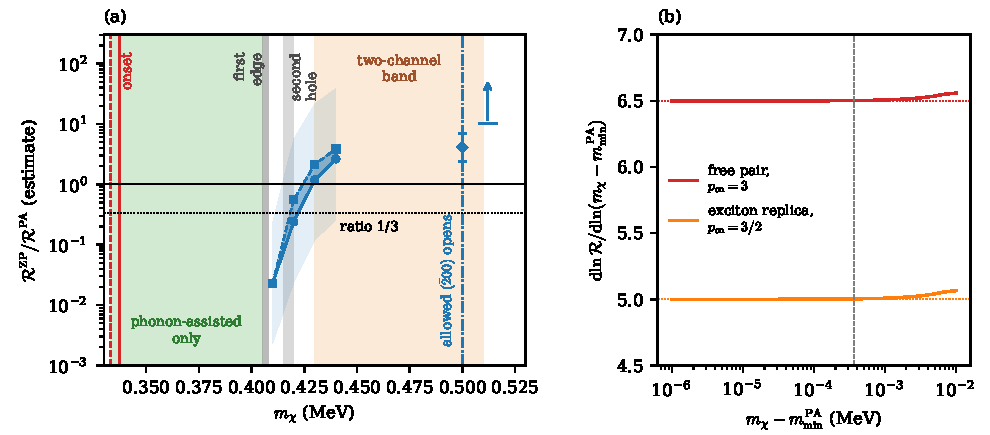
\includegraphics[width=\linewidth]{figures/ch13/fig13_9.pdf}
  \caption{Rates across the silicon window. (a)~Estimated ratio of the zero-phonon to the phonon-assisted electron-recoil rate against the dark-matter mass. Green band: phonon-assisted only, from the onsets (red: free pair \SI{0.3374}{MeV}, solid; exciton replica \SI{0.3332}{MeV}, dashed) to the first zero-phonon edge; gray bands: the first zero-phonon edge (0.405--\SI{0.408}{MeV}) and the edge of the second heavy hole (0.415--\SI{0.420}{MeV}). Blue points: the ratio with the second-hole edge at \SI{0.420}{MeV} (circles) and \SI{0.415}{MeV} (squares), each channel at the largest energy above the first edge that the mass reaches; dark band between them, light band the factor of ten of the phonon-assisted side. Diamond: the allowed $(\bar2\,0\,0)$ line at its opening, \SI{0.50}{MeV} (dash-dotted), with one or two conduction bands reached; bar and arrow: ratio of 10 or more from \SI{0.51}{MeV}. Black lines: ratio one and one third. Orange: the two-channel band. Estimates: phonon-assisted side from the measured cold absorption (\SI{20}{K} data~\cite{macfarlane1958fine}; the \SI{0.5}{K} fit of \cref{we:13-darkphoton-edge} changes the ratios by at most \SI{5}{\percent}) and a computed vertex form factor; zero-phonon side a Wannier--Mott continuum with computed vertices; between 0.44 and \SI{0.50}{MeV} no ratio has been evaluated. (b)~Local power of the model rate, $\dd\ln\mathcal{R}/\dd\ln(\mchi - m_{\mathrm{min}}^{\mathrm{PA}})$, for a loss function $Cx^{p_{\mathrm{on}}}$ above the computed transverse acoustic onset on the valley axis (PBE force constants of \cref{sec:5.2}), the standard halo (\cref{tab:1-shm}) and a heavy mediator, with the asymptotes $p_{\mathrm{on}} + 7/2$ of \cref{eq:13.9-medge} (dotted). Dashed: the mass at which the largest energy above threshold reaches \SI{1.3}{meV}, the end of the $x^3$ range of \cref{fig:13-paloss}.}
  \label{fig:13-window-rates}
\end{figure}

The phonon-assisted rate leads the electron recoil of silicon at least to about \SI{0.42}{MeV} and centrally to about \SI{0.43}{MeV}. From there to about \SI{0.51}{MeV} lies a two-channel band, in which the rates are comparable and neither can be quoted alone with confidence. Above about \SI{0.51}{MeV} the allowed zero-phonon line leads. The biases point both ways. The isotropic exciton mass underestimates the zero-phonon density of states by a factor 1.3 to 1.6, which makes the ratios too low. The form factor, more likely low than high, makes them too high; the second-hole vertex and the evaluation at the largest energy make the zero-phonon side an upper estimate. A rate computed from the amplitude on the same bins as the zero-phonon rate would settle all of it.

\subsection{Germanium and GaAs}\label{sec:13.9-ge-gaas}

The germanium window has a known lower end and an unknown upper end. Its onset, 0.2119 to \SI{0.2141}{MeV}, rests only on the gap, the position of L and the measured transverse acoustic branch (\cref{sec:13.1}); the computed PBE branch is \SI{13.5}{\percent} low at X and \SI{11.6}{\percent} low at L, so its $\omega_{\mathrm{TA}}(\vect{Q}^*) = \SI{6.70}{meV}$ on a $6^3$ grid is too soft by about as much. It places the onset at \SI{0.21380}{MeV} for a free pair and \SI{0.21264}{MeV} for the bound $1s$ exciton, with an estimated binding of \SI{4.0}{meV}. Both lie inside the bracket, and scaling the branch to the neutron data moves them by at most \SI{0.0003}{MeV}, so the softness does not reach the onset (\cref{app:E.14}). The zero-phonon edge is not known. PBE puts the conduction state at $\mathrm{\Gamma}$ below the L valley, so no scissor-corrected PBE calculation can locate it (\cref{app:E.1}), and the joint minimization on quasiparticle bands with spin--orbit coupling is open. The value \SI{0.32}{MeV} of \cref{sec:13.1}, from the parabola on the L axis, assumes a parabolic pair with the hole at $\mathrm{\Gamma}$, and it brackets the edge in neither direction. Only the joint minimum restricted to the axis, evaluated on the true bands, would be an upper value. The silicon result does not settle whether the germanium optimum leaves the axis. The [111] valley axis of germanium is already its heavy-hole direction, and the silicon optimum came from a hole moving into a flat direction away from the valley axis. What does carry over is that spin--orbit coupling must be in the bands, and that the hole must be free in the minimization. The selection rule differs as well. The mirror planes that contain a [111] axis are the diagonal planes of the $\{110\}$ family, which belong to $\bar43m$ and carry no fractional translation (\cref{app:C.17}); there is no glide phase, and on the L axis the vertex at the extrema does not vanish (\cref{sec:10.5-rules}). Whether the first zero-phonon state of germanium is weakly coupled has to be checked at its optimum. Until then germanium has a phonon-assisted onset, the onset exponent 3 for every branch (\cref{sec:13.3}), and no window.

GaAs is the control: a direct gap with its own phonon-assisted band, which in the parabolic description of the $\mathrm{\Gamma}$ pair runs from an onset of 0.433 to \SI{0.436}{MeV} to the opening of the zero-phonon channel through the L valleys, between 0.517 and \SI{0.560}{MeV} (\cref{sec:13.1}). Both ends of that bracket are rigorous for the given L energy; only the position of the edge between them needs bands. The top scales as $2E_{\mathrm{L}}/v_{\mathrm{max}}^2$, and for a detector the low-temperature L energy applies. That GaAs reproduces this band, and that its phonon-assisted rate is a small correction wherever a zero-phonon line is open, is the control that \cref{app:E.14} specifies.

\subsection{The silicon window in one table}\label{sec:13.9-table}

\Cref{tab:13-window} collects the window in two blocks: what two independent calculations or a symmetry argument with a numerical check establish, and what rests on one calculation or an estimate, or is open.

\begin{table}[tbp]
  \caption{The silicon window, with germanium and GaAs. Masses in MeV. Status: ``two independent calculations'', ``symmetry, confirmed numerically'', ``derivation'', ``one calculation'', ``measured data'', ``estimate'' (a model in which the phonon-assisted rate is known to a factor of ten either way, apart from the unsized pair channel), ``open''. Bands at the measured lattice constant with spin--orbit coupling, gap $\Eg(0) = \SI{1.170}{eV}$, halo of \cref{tab:1-shm}.}
  \label{tab:13-window}
  \centering\footnotesize\setlength{\tabcolsep}{3pt}
  \begin{tabular}{@{}>{\raggedright\arraybackslash}p{0.33\linewidth}>{\raggedright\arraybackslash}p{0.27\linewidth}>{\raggedright\arraybackslash}p{0.2\linewidth}>{\raggedright\arraybackslash}p{0.13\linewidth}@{}}
    \toprule
    Quantity & Value & Status & Section \\
    \midrule
    \multicolumn{4}{@{}l}{\emph{Established}} \\
    First zero-phonon edge, continuum & 0.405--0.408 (best 0.407); off the axis, $\{001\}$ mirror plane, tilt \SI{0.18}{rad} & two independent calculations & \cref{sec:13.9-edges} \\
    First zero-phonon edge, $1s$ line & 0.402--0.405 & two independent calculations & \cref{sec:13.9-edges} \\
    Second (mirror-even) heavy hole & from 0.415--0.420 & 0.415: two independent calculations; 0.420: estimate & \cref{sec:13.9-edges} \\
    Allowed $(\bar2\,0\,0)$ line opens & $\approx 0.50$ (X face); vertex at the class extremum $\sum_v|\rho_{cv}|^2 = 0.150$ & two independent calculations & \cref{sec:13.9-edges,sec:13.9-glide} \\
    Selection rule & first line second class by the glide; $(\bar2\,0\,0)$ class allowed; spin--orbit lift $3.6\times10^{-6}$ (axis), $1.3\times10^{-4}$ (plane) & symmetry, confirmed numerically & \cref{sec:13.9-glide} \\
    Order of the edges & onset $<$ first edge $<$ second hole $<$ allowed line & two independent calculations & \cref{sec:13.9-edges} \\
    \midrule
    \multicolumn{4}{@{}l}{\emph{Estimated or open}} \\
    Phonon-assisted onset & 0.3332 (exciton replica), 0.3374 (free pair) & one calculation & \cref{sec:13.1} \\
    Phonon-assisted rate leads & centrally to $\approx 0.43$ (0.424--0.428), at least to $\approx 0.42$ (0.418--0.421) & estimate & \cref{sec:13.9-rates} \\
    Two-channel band & 0.43--0.51 & estimate & \cref{sec:13.9-rates} \\
    Zero-phonon rate leads & above $\approx 0.51$ (ratio 2.4--7.0 at 0.50, $\ge 10$ pointwise from 0.51) & estimate & \cref{sec:13.9-rates} \\
    Screening correction relative to the optical calibration & 0.3--2.6 on $L^{\mathrm{PA}}$ (external factor and local-field wings); pair channel beyond the calibration not sized & estimate & \cref{sec:13.4,sec:13.9-rates} \\
    Rate and reach & $\sigmae \approx 3\times10^{-30}$--$3\times10^{-29}$ (0.36; the \SI{0.5}{K} fit extrapolated below \SI{1.206}{eV} carries half of it), $4\times10^{-32}\,\si{cm^2}$ (0.40), heavy mediator, \SI{1}{kg.yr}; power $p_{\mathrm{on}} + 7/2$ at the onset & estimate (factor 10 at 0.40; 15 at 0.36); power: derivation & \cref{sec:13.9-onset,sec:13.9-rates} \\
    Germanium & onset 0.2119--0.2141; zero-phonon edge not known & onset from measured data; edge open & \cref{sec:13.1,sec:13.9-ge-gaas} \\
    GaAs & phonon-assisted band 0.43 to 0.52--0.56 & estimate (parabolic $\mathrm{\Gamma}$ pair) & \cref{sec:13.1,sec:13.9-ge-gaas} \\
    \bottomrule
  \end{tabular}
\end{table}

\subsection{Nuisance table of the phonon-assisted sector}\label{sec:13.9-nuisances}

\Cref{tab:13-nuisances} collects the truncations and inputs of the chapter, each with its size and the section that treats it, in the classes of \cref{sec:8.8}.

\begin{table}[tbp]
  \caption{Nuisances of the phonon-assisted sector. Type in the classes of \cref{sec:8.8}: normalization, tilt (in $\omega$, in $q$ or in the dark-matter mass), threshold and new support. Basis of the size: ``computed'' (next order computed), ``model'' (next order computed in a model), ``est.''\ (parametric estimate), ``bound'' (only an inequality or two limits are known), ``named'' (no size). Sizes are for silicon unless another crystal is named. The last column gives the section where the item is treated.}
  \label{tab:13-nuisances}
  \centering\scriptsize\setlength{\tabcolsep}{3pt}
  \begin{tabular}{@{}>{\raggedright\arraybackslash}p{0.27\linewidth}>{\raggedright\arraybackslash}p{0.12\linewidth}>{\raggedright\arraybackslash}p{0.36\linewidth}>{\raggedright\arraybackslash}p{0.09\linewidth}>{\raggedright\arraybackslash}p{0.10\linewidth}@{}}
    \toprule
    Truncation or input & Type & Size & Basis & Section \\
    \midrule
    Transverse acoustic energy at $\vect{Q}^*$ (PBE branch \SI{8}{\percent} soft at X) & threshold & onset $+\SI{0.0004}{MeV}$ with the branch scaled to the neutron data; \SI{2.8e-4}{MeV} per meV & computed & \cref{sec:13.1} \\
    Exciton binding & threshold & phonon-assisted onset 0.3374 $\to$ \SI{0.3332}{MeV}; zero-phonon edge $-\SI{0.0028}{MeV}$ & computed & \cref{sec:13.1,sec:13.9} \\
    Fixed directions of $\vect{q}$, hole at the valence maximum & threshold & zero-phonon edge 0.405--0.408 against 0.420--\SI{0.425}{MeV} on the axis & computed & \cref{sec:13.1,sec:13.9} \\
    Spin--orbit coupling in the bands & threshold & first zero-phonon edge $+\SI{0.003}{MeV}$; on the axis $< \SI{0.0002}{MeV}$ & computed & \cref{sec:13.9} \\
    Band sum cut to empty bands & normali\-zation & $|M|^2$ off by a factor 1.6 to 2.4 in a two-band chain (two phase conventions of its phonon vertex) & model & \cref{sec:13.2} \\
    Adiabatic (Herzberg--Teller) amplitude & normali\-zation & \SI{1.6}{\percent} (TA), \SI{5.2}{\percent} (TO) at the edge; \SI{10}{\percent} when $E_{\mathrm{min}}(\vect{q}) - \omega$ falls to \SI{0.18}{eV} (TA) & est. & \cref{sec:13.2} \\
    Next order in the electron--phonon vertex ($n_g = 4$) & normali\-zation & $\theta_{\mathrm{ep}} = 0.010$--0.016 at the absorption edge; $\approx 0.2$ at the window edge & est.; bound & \cref{sec:13.3,sec:13.6} \\
    Tilt of the pair minimum, branch curvature & threshold & \SI{0.02}{meV} (TA), \SI{0.18}{meV} (LA) at \SI{1}{keV}; masses \SI{1}{\percent} & computed & \cref{sec:13.3} \\
    External screening $1/(\varepsilon_1^0)^2$ & normali\-zation & 1/30--1/38 at \SI{1}{keV}; 3.7--\SI{4.4}{\percent} across the window & computed & \cref{sec:13.4} \\
    Screening relative to the optical calibration: external model factor, local-field wings, pair channel & normali\-zation & 0.3--2.6 on $L^{\mathrm{PA}}$ for the external factor and the wings; pair ratio one in both solvable limits at exact pinning; residual from the \SI{0.2}{keV} spread of pair momenta and the range between the limits not sized & est.; named & \cref{sec:13.4,sec:13.9} \\
    Adiabatic local-density source & normali\-zation & about \SI{5}{\percent} of the pair term & est. & \cref{sec:13.4} \\
    Parabolic pockets, constant vertex (edge form) & tilt in $\omega$ & within \SI{15}{\percent} of the \SI{300}{K} data from 55 to \SI{490}{meV} above the gap; factor 2 at \SI{17}{meV} & computed & \cref{sec:13.5} \\
    Temperature of absorption data & tilt in $\omega$ & untransferred \SI{77}{K} data $\times2.3$--2.6, 1.7--1.9, 1.3--1.5, 1.1--1.3 at 15, 25, 50, \SI{100}{meV}; strength factor 0.88 (\SI{77}{K}), 0.61 (\SI{295}{K}); branch weights $\pm\SI{25}{\percent}$: $<\SI{1}{\percent}$ from \SI{77}{K} & computed & \cref{sec:13.5} \\
    Cold absorption data: \SI{0.5}{K} fit against \SI{20}{K} data & normali\-zation; tilt in $\omega$ & $\times20$ at \SI{1.20}{eV}, $\times2.1$ at \SI{1.25}{eV}, within \SI{5}{\percent} above \SI{1.37}{eV}; rate $\times9$ at \SI{0.36}{MeV}, $\times1.8$ at \SI{0.40}{MeV}; \SI{55}{\percent} of the \SI{0.36}{MeV} rate from the fit below its lowest data point & computed & \cref{sec:13.8,sec:13.9} \\
    Margin of the off-shell window, pair widths & tilt in $q$ & controlling ratios $\le 0.21$ at $\delta_{\mathrm{w}} = \SI{0.3}{eV}$; widths 3--\SI{21}{meV}; window to $|\vect{q}| = \SI{1.33}{keV}$ (parabolic), \SI{1.27}{keV} (computed bands) & est.; model & \cref{sec:13.6} \\
    Fano term & tilt & zero in Si and Ge; GaAs $\lesssim 0.3\varGamma/\delta_{\mathrm{F}}$, a few percent of first emissions moved & est. & \cref{sec:13.6} \\
    Nonadiabatic zero-point renormalization & threshold & \SI{8}{meV} on the gap; onset \SI{0.0023}{MeV} if the gap is built from a computed renormalization; with the measured gap only its variation across the zone, zero-phonon edge $\le\SI{0.002}{MeV}$ & computed; bound & \cref{sec:13.7} \\
    Exciton--phonon replicas beyond the two-pair sector & new support & no size & named & \cref{sec:13.8} \\
    Singlet against triplet pairs in axion-like absorption & normali\-zation & no pair channel in the triplet response, size not known; replica lines shifted by the exchange splitting, about $2\times10^{-3}$ of $E_x^b$ & named (open) & \cref{sec:13.8} \\
    Finite-$q$ form factor of the rate estimate & normali\-zation; tilt in $\mchi$ & factor 3; combined factor 6.5 at 0.38--\SI{0.43}{MeV}, quoted as 10 & est. & \cref{sec:13.9} \\
    Completeness of the plane-wave band sum ($f$-sum) & normali\-zation & 0.81 $\to$ 0.89 of $q^2/2m_e$ with 16 $\to$ 100 bands; nonlocal and truncation parts not separated & computed & \cref{sec:13.9} \\
    Zero-phonon side of the ratio (isotropic exciton mass, second-hole vertex) & normali\-zation & density of states low by 1.3--1.6; second-hole term an upper estimate & est. & \cref{sec:13.9} \\
    Spin--orbit lift of symmetry zeros & new support & zero-phonon ratio $\le 0.01$; longitudinal acoustic kink $<10^{-4}$ on the axis & computed; est. & \cref{sec:13.3,sec:13.9} \\
    \bottomrule
  \end{tabular}
\end{table}

For the rate in the window, three rows dominate: the finite-$q$ form factor of the estimate, a factor three either way and probably low; the screening correction relative to the optical calibration, whose pair-channel part no calculation sizes; and, near the onset, the spread of the cold data. Every threshold row is small in mass, a few thousandths of an MeV at most, and the order of the edges survives all of them together. What a threshold error costs, however, is not small near the onset, where \cref{eq:13.9-medge} raises it to the power $p_{\mathrm{on}} + 7/2$.

\subsection{Open problems}\label{sec:13.9-open}

The onset rests on one set of force constants, soft on exactly the branch that sets it, and a direct calculation of $\omega_{\mathrm{TA}}(\vect{Q}^*)$ at two lattice constants and with a second pseudopotential would verify it (\cref{app:E.14}). The end of the phonon-assisted lead, the width of the two-channel band and the mass from which the zero-phonon line leads follow from the ratio of the two rates computed on common bins, with the full amplitude on the phonon-assisted side and the mirror-plane cones, the second heavy hole and the X-face edge on the zero-phonon side (\cref{app:E.14}). The same calculation gives the rate and the reach with their controls: the optical limit, the symmetry zeros, the soft acoustic limit and the completeness of the band sum, whose plane-wave $f$-sum with a norm-conserving pseudopotential reaches 0.81 of $q^2/2m_e$ with 16 bands and 0.89 with 100 at $|\vect{q}| = 0.1$ to \SI{0.5}{\angstrom^{-1}}, the bands left out and the nonlocal term not yet separated. The pair channel beyond the optical calibration needs the supercell calculation of \cref{app:E.16}, with local fields in the supercell basis. Germanium needs quasiparticle bands with spin--orbit coupling for its zero-phonon edge and phonons that pass the neutron data on the transverse acoustic branch, and GaAs, the control of the whole chain, its band calculation and its rate with the polar vertex (\cref{app:E.14}).

One measurement would test the chain directly: the cold absorption edge of silicon within \SI{25}{meV} of its threshold, which no measurement at millikelvin temperatures covers. There the untransferred \SI{77}{K} data are off by more than a factor of two (\cref{sec:13.5}), and the two cold datasets of \cref{sec:13.9-rates} differ by a factor of twenty at \SI{1.20}{eV}.

\section*{Summary}

Dark matter lighter than about \SI{0.4}{MeV} cannot create an electron--hole pair in silicon on its own: where it deposits the gap it transfers about \SI{0.9}{keV}, and a pair with that momentum costs more than the gap. A phonon of about \SI{15}{meV} takes the missing crystal momentum (\cref{sec:13.1}). The lightest mass that creates a pair without a phonon is a joint minimum over the momentum transfer and the hole's crystal momentum. The lightest that creates one with a phonon is the kinematic floor with the gap raised by one phonon energy, at the wavevector the dark matter leaves for the phonon: \SI{0.3374}{MeV} for the free pair, \SI{0.3332}{MeV} for the exciton replica. The onset is insensitive to the band structure and rests on one phonon energy. Germanium has its onset at 0.212 to \SI{0.214}{MeV} from the measured transverse acoustic branch alone, and GaAs, though direct, has a phonon-assisted band of its own above \SI{0.433}{MeV}, because its light pair cannot absorb the momentum either.

The amplitude is of second order, one density vertex and one electron--phonon vertex on four paths (\cref{sec:13.2}). The exclusion principle turns the paths through filled states into exchange partners of the blocked ones, and on shell the amplitude becomes a one-electron sum over all bands, filled ones included; cutting it to empty bands is wrong by a factor of order one. The intraband terms cancel at $\vect{q} = 0$, so the amplitude starts at first order in $q$. It does not interfere with the zero-phonon line, whose final states have one phonon fewer. Its adiabatic form is the derivative of the zero-phonon transition density with respect to a frozen phonon, the Herzberg--Teller term, accurate to a few percent at the absorption edge.

Squared and summed, the amplitude gives the phonon-assisted structure factor and loss function, which enter the rate exactly as the zero-phonon ones do (\cref{sec:13.3}). Inside the off-shell window they are the whole electronic response; above the zero-phonon edge they add to it, and the $f$-sum rule they share forbids adding a bare zero-phonon rate to them without the renormalization of \cref{sec:13.7}. At its threshold the direction-averaged loss function rises as the cube of the energy above it, as the fourth power at the longitudinal acoustic kink, which a selection rule on the valley axis forbids, and as the power 3/2 for an exciton replica.

Screening acts on the density vertex and on the final pair (\cref{sec:13.4}). The external factor is one inverse macroscopic dielectric function for the whole amplitude, $1/30$ to $1/38$ in the loss function at \SI{1}{keV} in silicon, far from the optical $1/\varepsilon_\infty^2$. The pair channel screens at the pinned momentum of the final pair, the same for every $\vect{q}$; its size and sign are open, bracketed only by two solvable limits a factor of ten apart, and in both limits a measured optical edge calibrates it at every $\vect{q}$.

As $\vect{q} \to 0$ the loss function becomes phonon-assisted optical absorption, by the continuity equation applied to the second-order amplitude (\cref{sec:13.5}). The measured edge of silicon is its test: the Hall--Bardeen--Blatt form, with one fitted scale, lies within \SI{15}{\percent} of the \SI{300}{K} data over 55 to \SI{490}{meV} above the gap. Absorption data must be transferred to the temperature of a detector branch by branch. The inverse transfer is exact for branch-resolved spectra and ill-posed without them, and untransferred \SI{77}{K} data overstate the cold edge by more than a factor of two within 18 to \SI{23}{meV} of it.

Two kinds of small denominator threaten the amplitude (\cref{sec:13.6}). Soft acoustic phonons give finite amplitudes once the recoil, deformation and velocity terms of a Ward identity are kept, and inside the window the soft limit is never reached. Zero-phonon detunings fix the window. The phonon-assisted rate is a channel of its own only where every first-order transition is off shell by a margin, \SI{0.3}{eV} in silicon. The margin confines it to $|\vect{q}| \le \SI{1.33}{keV}$ on the valley axis in the parabolic description and \SI{1.27}{keV} with the computed bands. Beyond the window only totals are defined, with the Dyson convention, and the Fano term vanishes in silicon and germanium.

At finite temperature and zero point the bands are renormalized, and a special-displacement calculation contains the adiabatic sideband, which places the phonon-assisted onset one phonon energy too low (\cref{sec:13.7}). Between room temperature and \SI{10}{mK} the gap opens by \SI{46}{meV} and the onset moves from 0.324 to \SI{0.337}{MeV}; below a few kelvin the window does not move. The nonadiabatic part of the zero-point renormalization, \SI{8}{meV} on the silicon gap, is already in the measured gap, and only its variation across the zone, at most \SI{0.002}{MeV} on the zero-phonon edge, can move the window. Excitons with phonons add replica edges below the free-pair edges, each rising as a square root at fixed $\vect{q}$, with a completeness condition that reduces to the two-pair sector; at the optical edge of cold silicon they carry most of the absorption. The same vertices give the phonon-assisted absorption of dark photons, axion-like particles and scalars at the indirect edge; the dark photon has no new pair-plus-phonon amplitude at first order in its coupling (\cref{sec:13.8}).

In silicon the first zero-phonon edge lies at 0.405 to \SI{0.408}{MeV}, off the valley axis in a mirror plane, with its $1s$ line at 0.402 to \SI{0.405}{MeV} (\cref{sec:13.9}). The glide of the diamond structure forbids its vertex, so the first zero-phonon line is weak; the second heavy hole opens from 0.415 to \SI{0.420}{MeV}, and an allowed Umklapp line of full size opens at \SI{0.50}{MeV}, where the same glide inverts the rule. These edges, the rule and their order are established. Between the onset and the first edge the phonon-assisted rate is the only electron-recoil channel. Its rate rises from the onset as the power $p_{\mathrm{on}} + 7/2$ of the distance in mass, so that near the onset only the exponent is predicted. By an estimate normalized to the measured cold edge, with rates uncertain by a factor of ten apart from the pair channel's dependence on $q$, it leads to about \SI{0.43}{MeV}, the two channels share 0.43 to \SI{0.51}{MeV}, and the zero-phonon line leads above. The nuisances of the chapter are collected in \cref{tab:13-nuisances}. Germanium and GaAs need quasiparticle band calculations. Throughout, the dark matter coupled to the electron density, which does not act on spin; \cref{chap:14} turns to couplings that reach the spins of a magnet.
